\documentclass{standalone}
\usepackage{tikz}
\usepackage{verbatim}
\usetikzlibrary{positioning}
\begin{document}
\pagestyle{empty}
  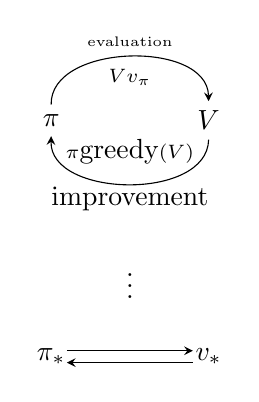
\begin{tikzpicture}
    \node (pi) at (-1, 0) {$\pi$};
    \node (v)  at ( 1, 0) {$V$};
    \path[-stealth] (pi) edge[bend left = 90] (v);
    \path[-stealth] (v)  edge[bend left = 90] (pi);
    \node at (0, 1) {\tiny evaluation};
    \node at (0, 0.55) {$\scriptstyle V v_\pi$};
    \node at (0, -0.4) {$\scriptstyle \pi\textrm{greedy}(V)$};
    \node at (0, -1) {improvement};
    \node at (0, -2) {$\vdots$};
    \node (pistar) at (-1, -3) {$\pi_*$};
    \node (pistar) at (1, -3) {$v_*$};
    \draw[-stealth] (-.8, -2.925) -- (.8, -2.925);
    \draw[stealth-] (-.8, -3.075) -- (.8, -3.075);
  \end{tikzpicture}
\end{document}